\documentclass[british]{article}
\usepackage{default}

\title{Unsupervised Learning}
\subtitle{IN3050V22 --- Assignment 3}
\author{%
  Martin Mihle Nygaard
  \textsf{\href{mailto:martimn@ifi.uio.no}{<martimn@ifi.uio.no>}}
}

\newcommand{\pca}{\texorpdfstring{\textsc{pca}}{PCA}}
\newcommand{\Cov}{\mathrm{Cov}\!\del}
\newcommand{\E}{E\!\sbr}

\begin{document}

\maketitle

\renewcommand{\abstractname}{Readme}
\begin{abstract}
  \noindent
  This one was pretty straight forward, as the guts of the code is spelled out
  in the Marsland book. I spent about 10\% of the time making the code work,
  10\% cleaning it up, and 80\% making the plots pretty\footnote{Essentially
  emulating Seaborn, I belatedly realised.}. Jupyter Notebooks still feel like
  bloat to me, so this is all Python + \textsc{pdf}. Hopefully this report
  answers the all the assignment questions and \textsc{rfc}s.

  \hbox

  \noindent
  The attached scripts \texttt{pca.py} and \texttt{kmeans.py} should reproduce
  the figures, and pass the test cases. I quote some of the code here, but it's
  not meant to run standalone (lacking proper imports and such), only to aid
  your assessment. I have also not commented on my plotting code.
\end{abstract}

% 1.
\section{Principal Component Analysis (\pca)}

\marginnote{What is the variance?} The \emph{variance} is a measure of how
spread out the data is; how far apart each data point is. This is calculated by
the average square deviation from the mean $\mu$, i.e.~$\sum_{i=1}^N
\del{x_i-\mu}^2 / N$, with $N$ as the number of data points. There is some
nuance here, though. What I just described is the \emph{population} variance
$\sigma^2$, and is correct if our data is finite and captures the entire
population \autocite[35]{devore-berk}.

I would imagine it is usually the case in unsupervised learning applications
that our data is a just a sample from greater population, that we assume is
somewhat randomly distributed. Then we would prefer to use the \emph{sample
variance} $s^2 = \sum_{i=1}^n \del{x_i-\bar x}^2 / \del{n - 1}$, where $n$ is
the number of samples, and $\bar x$ is their mean. The divisor in this formula,
$n-1$, is our \enquote{degrees of freedom} \autocite[34,35]{devore-berk}. 

In \emph{Numpy} the variance is by default calculated with zero \enquote{delta
degrees of freedom} (\textsc{ddof}), a divisor of $N-0$, that is
\autocite[\texttt{numpy.var}]{np}. In Python terms:
\begin{lstlisting}[numbers=none]
mean = lambda x: x.sum() / (len(x) - ddof)
var  = lambda x: mean(abs(x-mean(x))**2))
\end{lstlisting}

\marginnote{What is the covariance?} The \emph{covariance} is a measure of how
strongly related, or dependent, two (random) variables are to each
other. It is defined as \autocites[32]{marsland}[247]{devore-berk}\footnote{I
suspect there is a typo in \citeauthor{marsland}, as he suggest
$\Cov{X,Y} = \E{\del{X-\mu_X}}\E{\del{Y-\mu_Y}}$, in
contradiction to how he uses it in the covariance matrix on the next page,
where he uses \citeauthor{devore-berk}s definition instead.}:
$$ \Cov{X,Y} = \E{\del{X-\mu_X}\del{Y-\mu_Y}} $$
The sign of the covariance is indicative of the variables relationship: if
$\del{X-\mu_X}$ and $\del{Y-\mu_Y}$ tends in opposite directions, there is a
negative relationship; if they share sign, the covariance and relationship will
be positive. The magnitude of $\Cov{X,Y}$ is difficult to interpret
unless the variables are normalized. Also, notice that $$\Cov{X,X} =
\E{\del{X-\mu_X}^2} = \mathrm{Var}\!\del{X}.$$

\marginnote{How do we compute the covariance matrix?} If we let $\mathbf X$ be
a $N$-dimentional vector of data points such that $\mathbf X = \sbr{x_1, x_2,
\ldots, x_N}^T$, then the elements of the \emph{covariance matrix}
$\Cov{\mathbf X}_{ij}$ is simply the covariances of each pair points, $x_i$ and
$x_j$. You can also simplify this with some matrix operations, where
$E\!\cbr{\cdot}$ indicates element wise expected value
\autocites[33]{marsland}[711]{devore-berk}:
\begin{align*}
  \Cov{\mathbf X} &=
  \begin{bmatrix}
    \Cov{x_1,x_1} & \Cov{x_1,x_2} & \dots  & \Cov{x_1,x_N} \\
    \Cov{x_2,x_1} & \Cov{x_2,x_2} & \dots  & \Cov{x_1,x_N} \\
    \vdots        & \vdots        & \ddots & \vdots        \\
    \Cov{x_N,x_1} & \Cov{x_N,x_2} & \dots  & \Cov{x_N,x_N}
  \end{bmatrix} \\
  &=
  \begin{bmatrix}
    \E{\del{x_1-\mu_1}\del{x_1-\mu_1}} & \dots  & \E[1]{\del{x_1-\mu_1}\del{x_N-\mu_N}} \\
    \vdots                             & \ddots & \vdots                                \\
    \E{\del{x_N-\mu_N}\del{x_1-\mu_1}} & \dots  & \E[1]{\del{x_N-\mu_N}\del{x_N-\mu_N}}
  \end{bmatrix} \\
  &= E\!
  \left\{
  \begin{matrix}
    \begin{bmatrix}
      \del{x_1-\mu_1} \\ \del{x_2-\mu_2} \\ \vdots \\ \del{x_N-\mu_N}
    \end{bmatrix}
    \begin{bmatrix}
      \del{x_1-\mu_1} & \del{x_2-\mu_2} & \dots  & \del{x_N-\mu_N}
    \end{bmatrix}
  \end{matrix}
  \right\} \\
  &= E\!\cbr{\del{\mathbf X - \mu_{\mathbf X}}\del{\mathbf X - \mu_{\mathbf X}}^T}
\end{align*}

The covariance definition is somewhat muddied when we again consider our data
as samples from a greater population: the expected value, $\E{\cdot}$, is not
simply the arithmetic mean. We get a better guess of the covariance with a
\textsc{ddof} of 1; the \emph{sample covariance} formula for each $jk$-entry in
the matrix becoming \autocite{wiki-sample}:
$$ \Cov{\mathbf X}_{jk}=\frac{1}{N-1}\sum_{i=1}^{N} \del{x_{ij}-\bar{x}_j} \del{x_{ik}-\bar{x}_k}.$$
And, indeed, this is the default in \emph{Numpy}'s implementation
\autocite[\texttt{numpy.cov}]{np}.


\marginnote{What is the meaning of the principle of maximum variance?} In \pca\
a \emph{principal component} is a direction (vector) in the data with the
largest variation \autocite[134]{marsland}. This is the direction which,
hopefully, contains the most relevant information needed to separate the data,
since variation is usually what we use when we want to make classifications.
\marginnote{Why do we need this principle?} This is a nice way filter out
dimensions with little information, potentially also reducing noise.

\marginnote{Does the principle always apply?} \pca\ is by no means fail proof,
though; the direction with the most variation is not guarantied to contain the
signal we are looking for, maybe we even end up filtering out the relevant axis
since there happened to be some irrelevant, but extreme, variation in another
direction. This is whats happening in \autoref{fig:143}: the direction with the
most variablity does not help us classify the data points, but there is a clear
structure pressent (here captured by the second principal component).

% 1.2
\subsection{Implementation: How Is \pca\ Implemented?}

See the source files for the full implementation, but the vitals are quoted
below.

\marginnote{Centering the Data, \and Computing Covariance Matrix, \and
Computing Eigenvalues and Eigenvectors, \and Sorting Eigenvalues and
Eigenvectors} In the implementation of the helper functions, I've closely
followed the book \autocite[136--37]{marsland}. They are reduced to
one-liners, but are essentially the same.

\lstinputlisting[linerange={22-33}]{../src/pca.py}

% 1.2.6
\marginnote{\pca\ Algorithm}

For the main algorithm, see code below. Again, pretty much copied the book here
\autocite[136--37]{marsland}, though some changes: The algorithm is
refactored into several functions, as per assignment specification; and the
vectors are \emph{not} normalized, since the assignment tests apparently are
not, too.

\lstinputlisting[linerange=34-40]{../src/pca.py}

All functions in this section should pass the test cases from the assignment
text without issue.

% 1.3
\subsection{Understanding: How Does \pca\ Work?}

% 1.3.5
\marginnote{Visualize the \pca\ Projection}

I've visualized the original iris data, the centered data, the principal
eigenvector, and its one-dimensional projection in \autoref{fig:135}. Plotting
code is always an ugly mess, so see \texttt{pca.py} for implementation details.

\begin{figure}
  \centering
  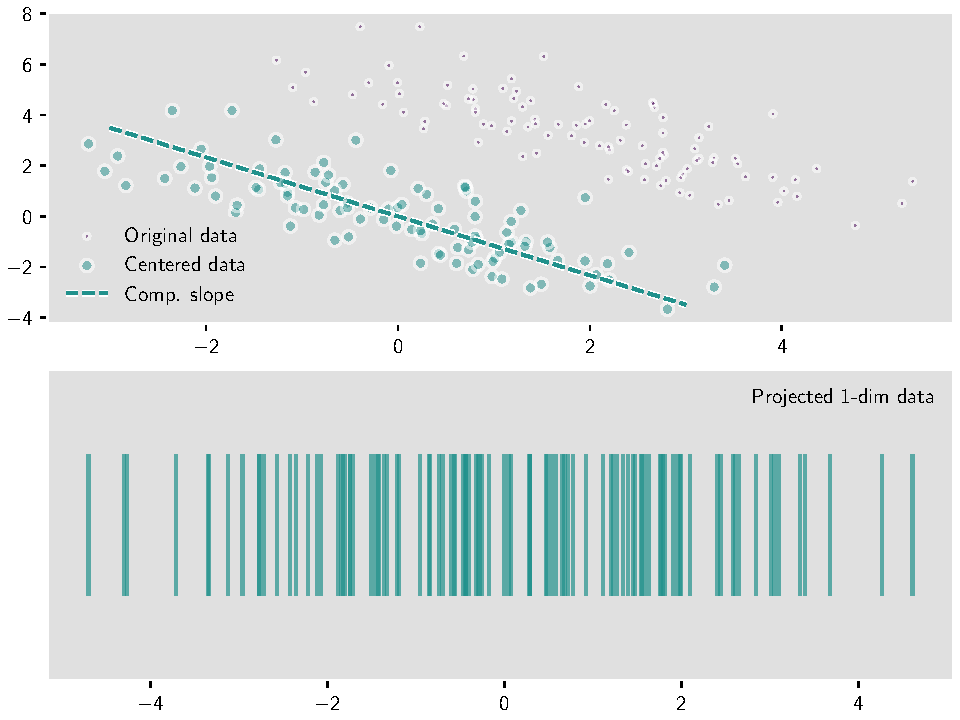
\includegraphics[width=0.9\columnwidth]{fig/135.pdf}
  \caption{Visualizing \pca.}
  \label{fig:135}
\end{figure}


% 1.4
\subsection{Evaluation: When Are the Results of \pca\ Sensible?}

% 1.4.2
\marginnote{Running \pca\ with Labels}

\begin{figure}
  \centering
  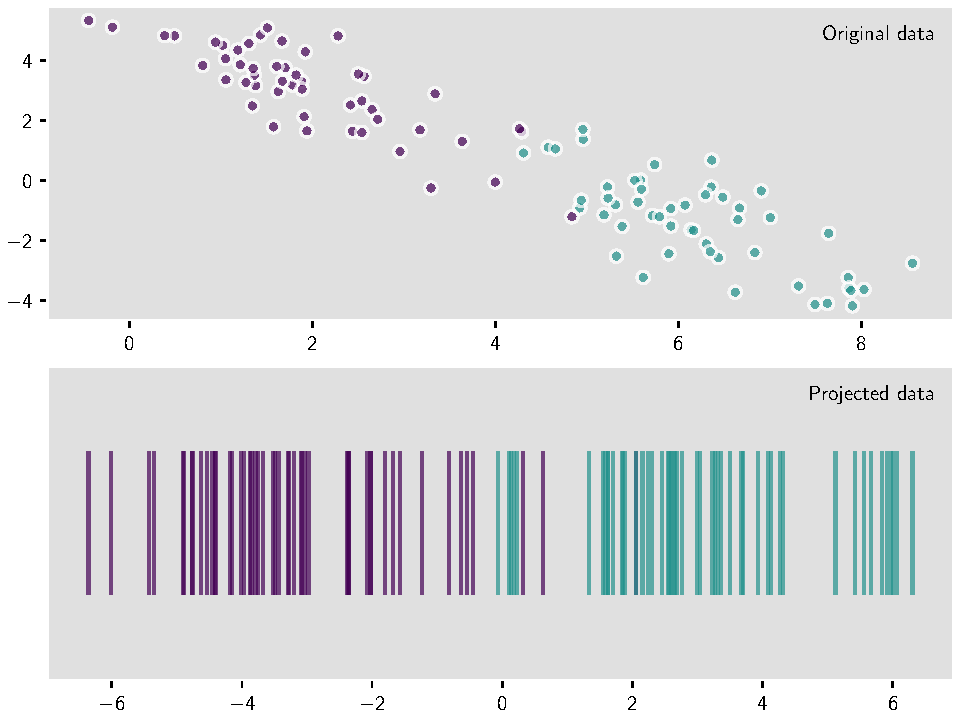
\includegraphics[width=0.9\columnwidth]{fig/142.pdf}
  \caption{Visualizing \pca\ with labeled data (1)}
  \label{fig:142}
\end{figure}

See \autoref{fig:142} for a visual of both the original data and the
principal component projected to one dimension. The data is now centered
around the origin, and is one-dimensional. It seems the information
necessary to separate the labels is preserved. The variability
perpendicular to the principal component looks like noise, and would
probably just make a classifier overfit.

% 1.4.3
\marginnote{Loading the Second Set of Labels}

In \autoref{fig:143} I've plotted the data with the second set of
labels. Both before and after doing \pca. I've plotted 2
components here. The first component, the one with most variability, is
not suitable for separating the two classes, but the second one is---not
\emph{perfect} by any means, but better. Using both could potentially
yield even better results, but might overfit if not careful, I think,
since the data appears rather noisy.

\begin{figure}
  \centering
  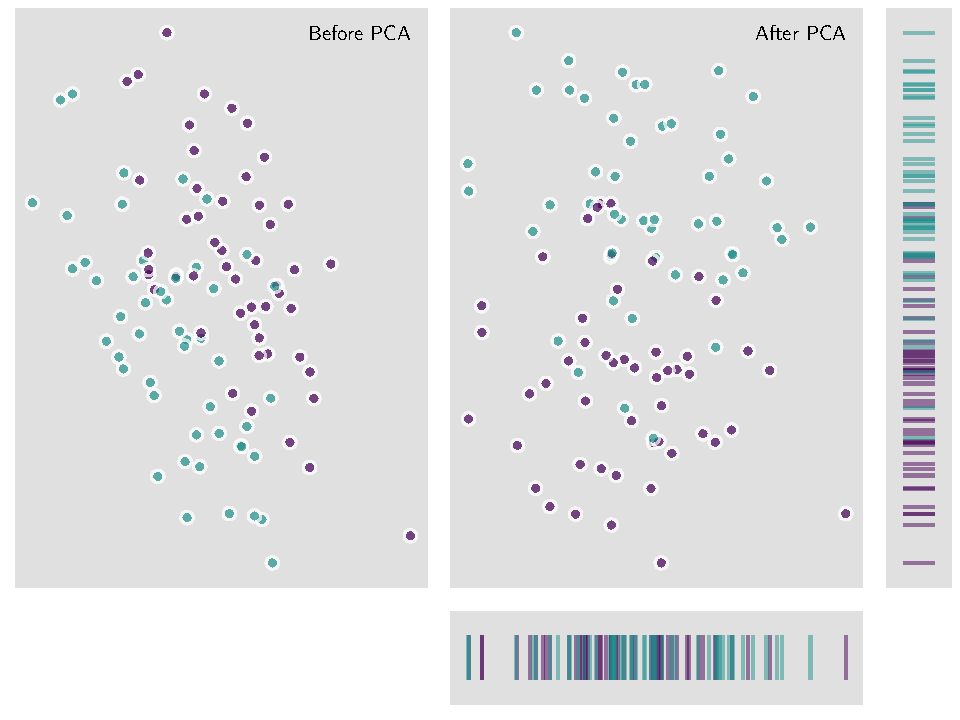
\includegraphics[width=0.9\columnwidth]{fig/143.pdf}
  \caption{Visualizing \pca\ with labeled data (2)}
  \label{fig:143}
\end{figure}

% 1.5
\subsection{Case Study 1: \pca\ for Visualization}

% 1.5.2
\marginnote{Visualizing the Data by Selecting Features}

In \autoref{fig:152} I've presented a scatter plot matrix of all the
iris features in the data set, with histograms on the diagonal.

\begin{figure}
  \centering
  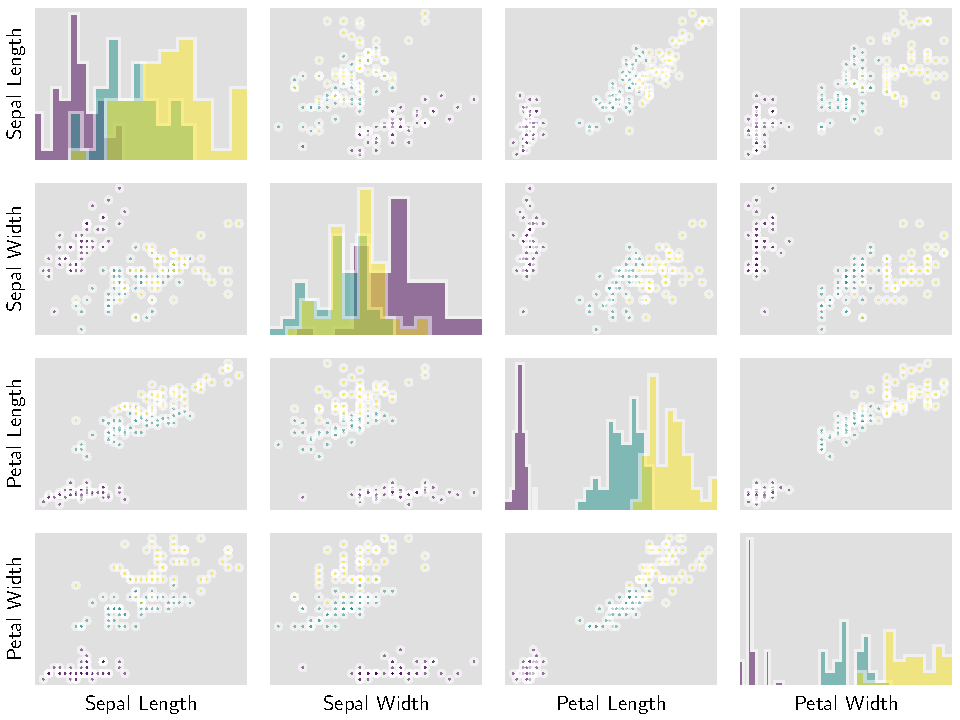
\includegraphics[width=0.9\columnwidth]{fig/152.pdf}
  \caption{Scatter plot matrix of iris dataset features}
  \label{fig:152}
\end{figure}

% 1.5.3
\marginnote{Visualizing the Data by \pca}

In \autoref{fig:153} I've plotted the 4 principal components of the dataset.
Also, see \autoref{fig:203} for a \textsc{\oldstylenums{2}d} representation of the first and second
principal components. Honestly, unless I've made some mistake, visualizing by
selecting features is much more informative for me. The first component
contains useful information for sure (the others less so), but it is difficult
to interpret. Whereas in the previous plot, I'm able to tell \emph{why} an iris
is classified the way it is.

\begin{figure}
  \centering
  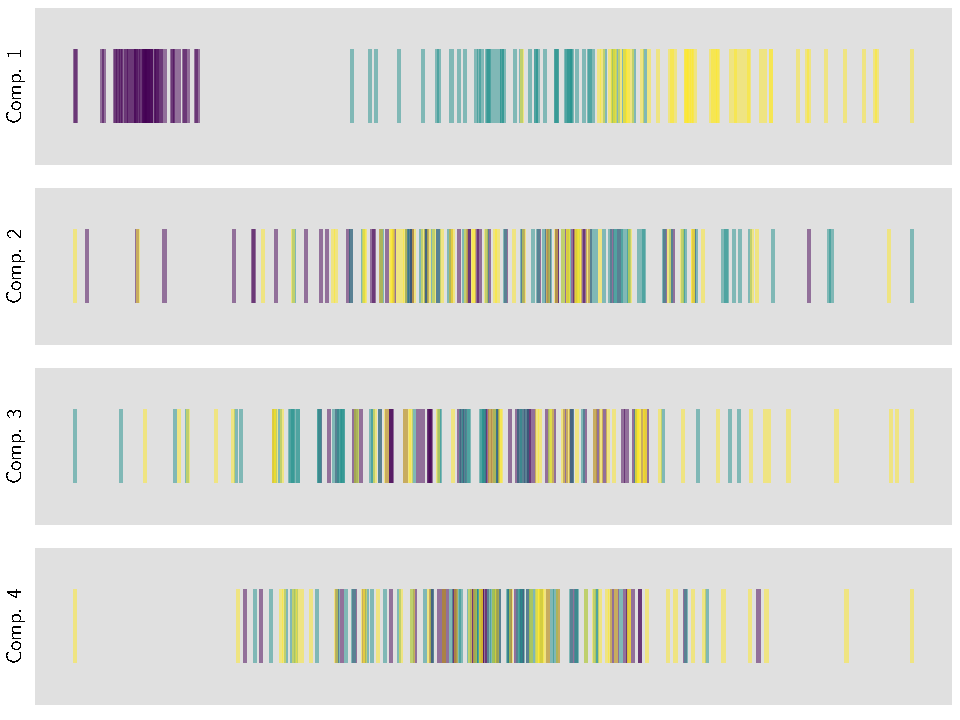
\includegraphics[width=0.9\columnwidth]{fig/153.pdf}
  \caption{Visualizing iris dataset using \pca}
  \label{fig:153}
\end{figure}

% 1.6
\subsection{Case Study 2: \pca\ for Compression}

% 1.6.1
% \marginnote{Loading the Data}

% 1.6.2
\marginnote{Inspecting the Data}

A sample image (the first) from the \emph{Faces in the Wild} dataset is shown
in \autoref{fig:162}.

\begin{figure}
  \centering
  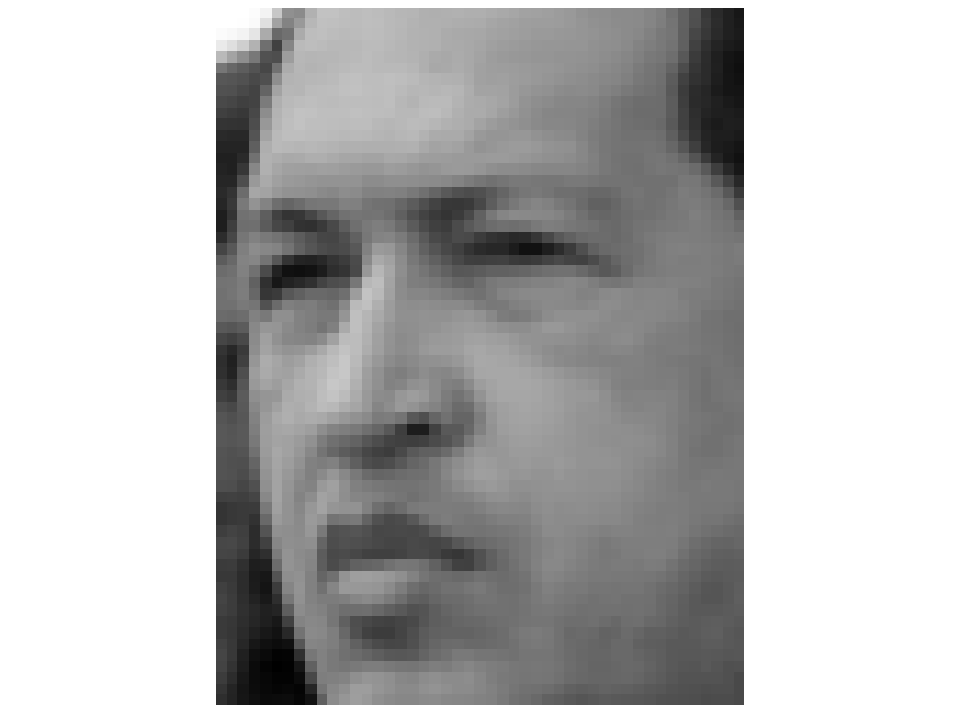
\includegraphics[width=0.9\columnwidth]{fig/162.pdf}
  \caption{Sample image (uncompressed)}
  \label{fig:162}
\end{figure}

% 1.6.3
\marginnote{Implementing a Compression-Decompression Function}

I've followed the algorithm in \cite[page 137]{marsland}, but I had to do an
additional transpose of the encoded matrix to line up the dimensions properly.
I also used the matrix multiplier \enquote{\texttt @}, instead of the dot
product, since it produces the same results in this case\footnote{Not sure why,
though.}. See the function definition below (from \texttt{pca.py}):

\lstinputlisting[linerange=42-43]{../src/pca.py}

% 1.6.4
% \marginnote{Compressing and Decompressing the Data}

% 1.6.5
\marginnote{Inspecting the Reconstructed Data}

5 samples of images from data compressed down to 200 dimensions, then
decompressed back to the original amount, is shown in \autoref{fig:165}. It
works surprisingly well, actually, considering the compressed data is
approx.~$200/2914 \approx 6.9\%$ of the original---if you disregard the vectors
needed to apply the (de)compression, that is.

\begin{figure}
  \centering
  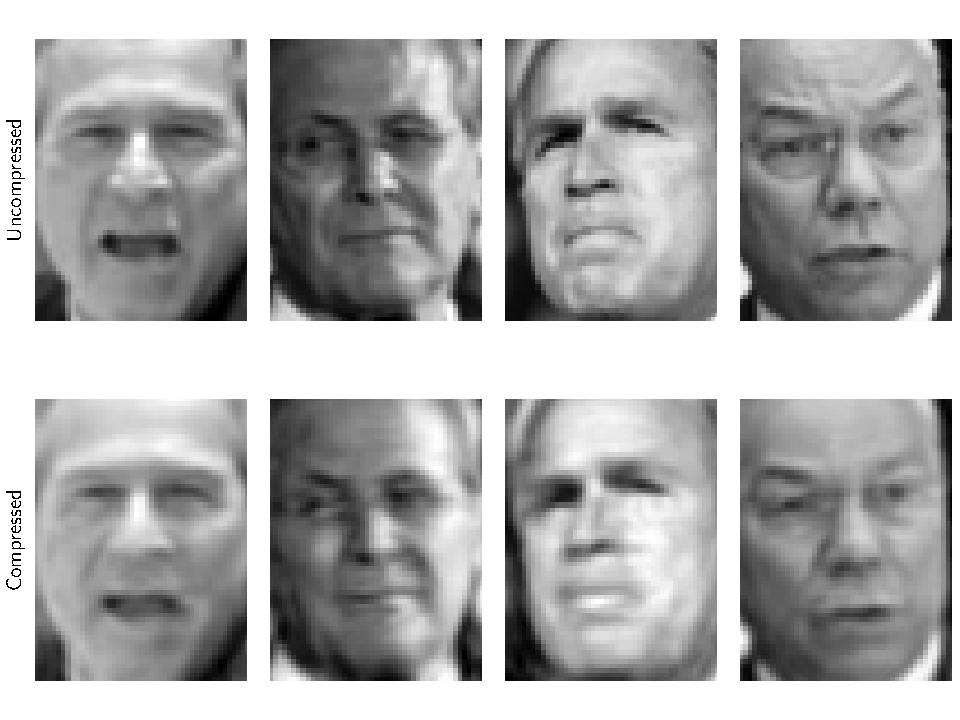
\includegraphics[width=0.9\columnwidth]{fig/165.pdf}
  \caption{Compressed--decompressed images using \pca, 200 dimensions}
  \label{fig:165}
\end{figure}

% 1.6.6
\marginnote{Evaluating Different Compressions}

\autoref{fig:166} shows examples of images from dataset compressed down to $m$
dimensions, with $m \in \cbr{100, 200, 500, 1000}$, then decompressed back to
the original. I find it difficult to spot any difference between the originals
and 1000 dimension compression. Even at 500 I have to squint to notice some
slight changes in texture. At 200 dimension compression, though, it's really
noticeable: sharp lines gets smoothed, textures scrambled, and some details
disappears entirely. 100 is worse, but the essence of the original is still
there. I think the 6th column from the right is interesting: the original
picture almost in profile, the face slightly turned; but it looks like with
heavier compression, the face turns more and more towards the camera, and the
background gets reinterpreted as part of the face. I'm guessing this is because
the original camera angle is novel, and in lower dimensions is discarded as
“noise”.

\begin{figure}
  \centering
  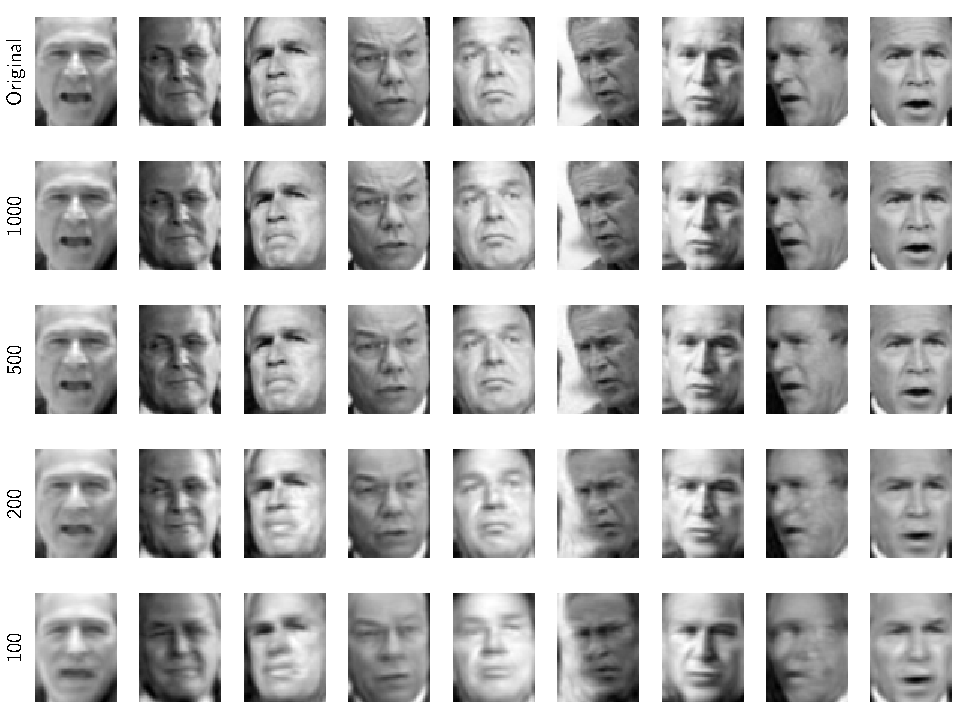
\includegraphics[width=0.9\columnwidth]{fig/166.pdf}
  \caption{Compressed--decompressed images using \pca}
  \label{fig:166}
\end{figure}


% 2.
\section{\emph{k}-Means Clustering}

See \texttt{kmeans.py} for the full script.

\subsection{Qualitative Assessment}

% 2.0.3
\marginnote{Projecting the Data Using \pca}
A plot of the original data with the \enquote{true} labels, along with 2
principal components, are shown in \autoref{fig:203}.

\begin{figure}
  \centering
  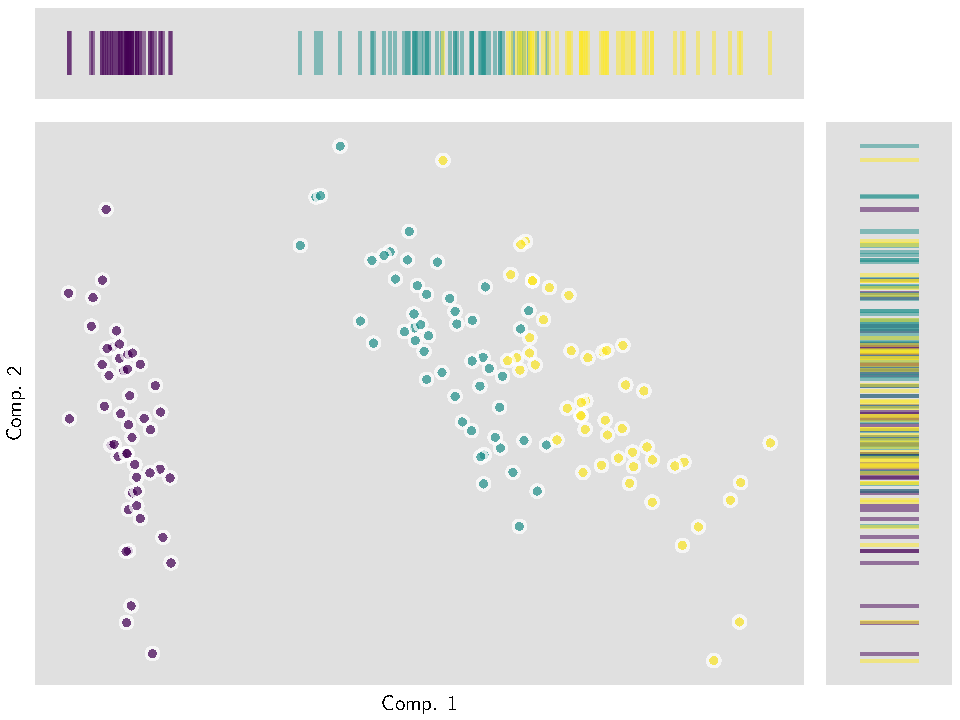
\includegraphics[width=0.9\columnwidth]{fig/203.pdf}
  \caption{\pca\ on iris dataset}
  \label{fig:203}
\end{figure}

% 2.0.4
\marginnote{Running \emph k-means}\label{sec:run-kmeans}
I do the $k$-means clustering for $k \in \cbr{2, 3, 4, 5}$ like so\footnote{
  I'm wondering: why would I use $\mathbf P$, the projection, and not
  $\mathbf X$, the original data, here? Doesn't $\mathbf X$ contain more
  information for the $k$-means algorithm to detect? Or would this just be
noise?}:

\lstinputlisting[linerange={38-39}]{../src/kmeans.py}

\begin{figure}
  \centering
  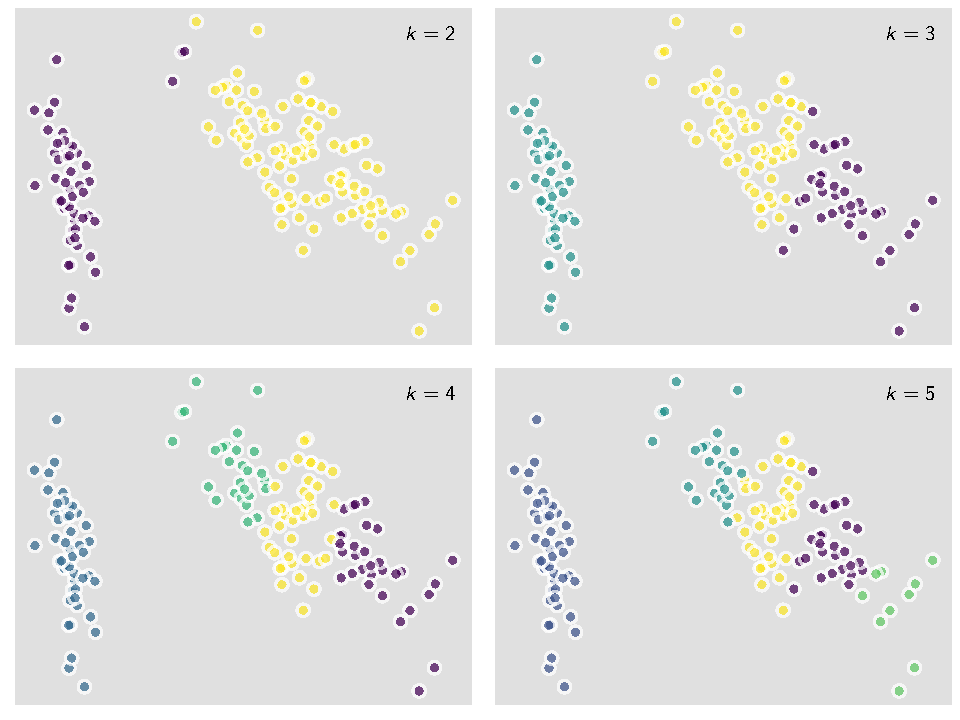
\includegraphics[width=0.9\columnwidth]{fig/205.pdf}
  \caption{$k$-means clustering on iris dataset}
  \label{fig:205}
\end{figure}

% 2.0.5
% \marginnote{Qualitative assessment}
Plots of the resulting labels are shown in \autoref{fig:205}. The $k$-means
predictions are not \emph{too} bad. Especially for $k=3$: though the boundary
between class 1 and 2 (as $y$ labels them) is not correct, it is not far off,
and---in my opinion---looks smoother than the \enquote{correct} $y$ labeling.
There are some minor, but glaring and annoying, \enquote{mistakes} (at least by
human standards) in the $k=2$ case. For $k \in \{4, 5\}$ the clustering seems
also logical, if there actually was more classes.

% 3.
\subsection{Quantitative Assessment}

First, I find the accuracy of a classifier trained on the true labels:
\lstinputlisting[linerange={60-60}]{../src/kmeans.py}

I train new classifiers on the $k$-means output from the previous section: (1)
one-hot-encode, (2) fit classifiers, and (3) measure accuracy.
\lstinputlisting[linerange={66-68}]{../src/kmeans.py}

\begin{figure}
  \centering
  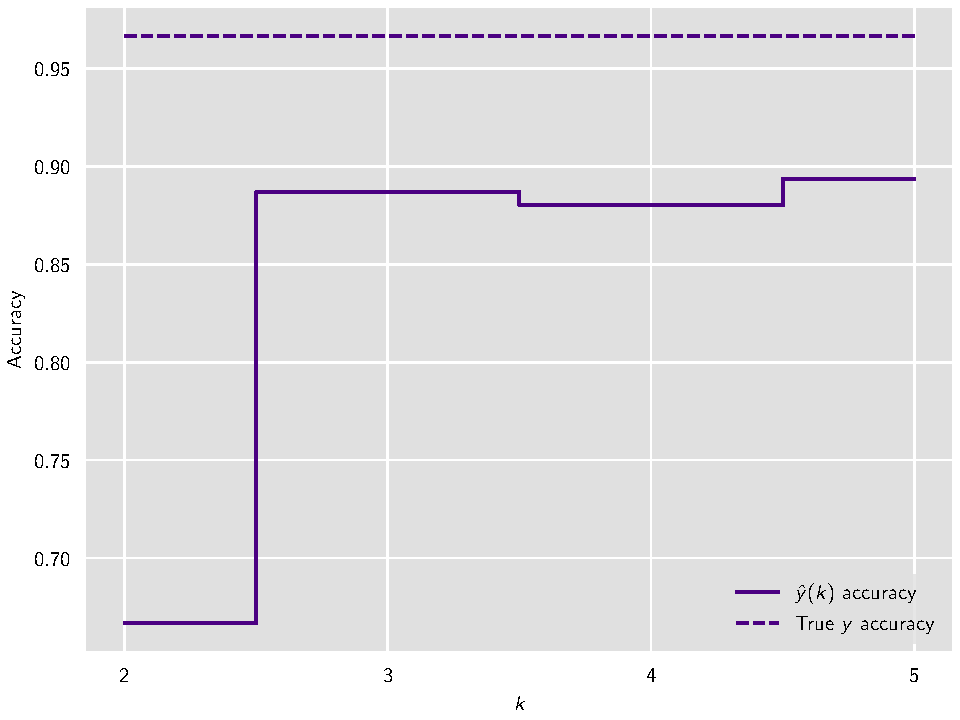
\includegraphics[width=0.9\columnwidth]{fig/300.pdf}
  \caption{Accuracy of logistic classifiers trained on $k$-means output}
  \label{fig:300}
\end{figure}

The accuracy results are shown in \autoref{fig:300}.

\printbibliography

\end{document}
